\chapter{Tecniche e Framework utilizzati}

\section{Version Control System}

Per controllare il versionamento del software durante tutta la fase di sviluppo è stato utilizzato il software \textsl{git}, in congiunzione con la piattaforma \textsl{github}:
\begin{itemize}
	\item[Maven -] https://github.com/FrancescoTerrosi/rehearsal-room-project
	\item[Gradle -] https://github.com/FrancescoTerrosi/rehearsal-room-gradle
\end{itemize}

Nonostante il lavoro sia stato svolto da un singolo studente è stato comunque adottato il modello \textsl{gitflow}, accompagnato dai meccanismi di pull-request offerti da \textsl{github}, grazie ai quali è stato possibile effettuare vari check di integrità della build su \textsl{travis}, \textsl{coveralls} e \textsl{sonarcloud}.

\section{Build Automation}

Come già detto, sono stati usati due strumenti di build automation:
\begin{itemize}
	\item Maven: solido, conosciuto e ben accettato nell'ambiente di sviluppo software, data la sua diffusione vi sono molti tutorial, plugin e schemi di configurazione
	\item Gradle: molto recente, in continuo sviluppo, permette una configurazione pressoché totale della build del progetto
\end{itemize}

\subsection{Maven}

Le specifiche di un progetto Maven vengono definite nel file "pom.xml".\newline
All'interno di questo file è possibile definire alcune opzioni di configurazione del progetto (nome del gruppo e del progetto, versione di Java\dots) e, soprattutto, definire le dipendenze necessarie al corretto funzionamento del software e plugin che specificano le operazioni da fare durante il processo di build.\newline
Per adottare una sorta di approccio modulare anche nel processo di build del progetto, sono stati definiti diversi profili all'interno del pom.\newline
Definire un profilo permette di incapsulare i plugin e le loro configurazioni al suo interno, in modo tale che queste vengano attaccate alla fase appropriata del lifecycle di Maven solamente quando richiesto.\newline
Per separare le operazione di generazione dei report di \textsl{JaCoCo}, i \textsl{Mutation Tests}, gli \textsl{Integration Tests} e gli \textsl{End to End Tests} sono stati quindi definiti i profili:
\begin{itemize}
	\item jacoco
	\item mutation
	\item integration
	\item e2e
\end{itemize}

\begin{minipage}{\linewidth}
	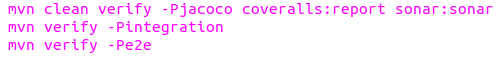
\includegraphics[width=\textwidth]{img/maven-goals.png}
	\captionof{figure}{Fasi e profili utilizzati per effettuare la build del progetto su travis-ci. Il profilo \textsl{mutation} non viene utilizzato in quanto di scarsa rilevanza per i check successivi (ma molto utile in locale)}
\end{minipage}
\newline

